%% !TEX root =  paper.tex
\section{Approach}\label{sec:approach}

The goal of our approach is to
detect and find potential fixes to locator problems that pertain to the breakage scenarios described in \autoref{sec:breakage-scenarios}.
%
%that can repair a broken web test that used to work correctly on a version $V$ of the AUT, and that now breaks when applied on a subsequent version $V+n$ (with usually $n=1$).
%
%The focus of our technique is to repair \textit{locators}, that represent the main source of breakage.
%Our technique can detect and correct locator problems that pertain to the breakage scenarios described in \autoref{sec:breakage-scenarios}.
In a nutshell, we capture the execution trace of each test statement for a version $V$ and use it to assert its correctness (or repair it) when executed on a subsequent version $V+n$ ($n \geq 1$). 
%Whenever possible, our technique attempts to repair breakages automatically, but also logs each encountered breakage or in inconsistency. 
% However, a detailed log of the encountered breakages is kept, so as to warn the developer of potential inconsistencies or breakages, and create potential candidate repairs to fix them. 

\autoref{approach} illustrates the usage scenario for our approach, which requires a correct version of the web application $V$ along with its working test suite $TS$ (i.e., in which all tests pass)~\ding{182}. 
A tester would run $TS$ by means of the first module of the presented approach~\ding{183}. Such a module collects, for each test, a variety of information (e.g., screenshots, DOMs)~\ding{184}. 
Then, as the application $V$ evolves into a new version $V'$ ~\ding{185}, a tester may wish to use $TS$ to check if regressions have occurred. The tester would use the second module of our approach~\ding{186} which runs each test case of $TS$ against the new version $V'$, and makes use of the information about the previous execution traces to \textit{verify and validate} the feasibility of each test statement, and eventually attempt to search for candidate repairs that can fix the locator breakages. At the end of the process, the approach outputs the validated (and eventually repaired) test suite $TS'$ that works on $V'$, together with report information. 
The tester can then manually analyze the report along with the repaired test cases. $TS'$ now represents a working test suite for the version $V'$ which can be used as a baseline for our approach when $V'$ will evolve further. 
The manual effort required is potentially significantly reduced in comparison to a user carefully verifying each executing test and manually searching for fixes as breakages occur. %
We now detail each step of our approach. 

\subsection{Execution Trace Collection}
%
In the first part of our approach, we capture a model of the runtime execution of the test cases, which we refer to as \textit{dynamic visual execution trace}.
Such a model comprises a sequence of test states, where each test state captures the DOM and visual information associated with each test statement of each test case. 

\begin{figure}[t]
\centering
%\fbox{
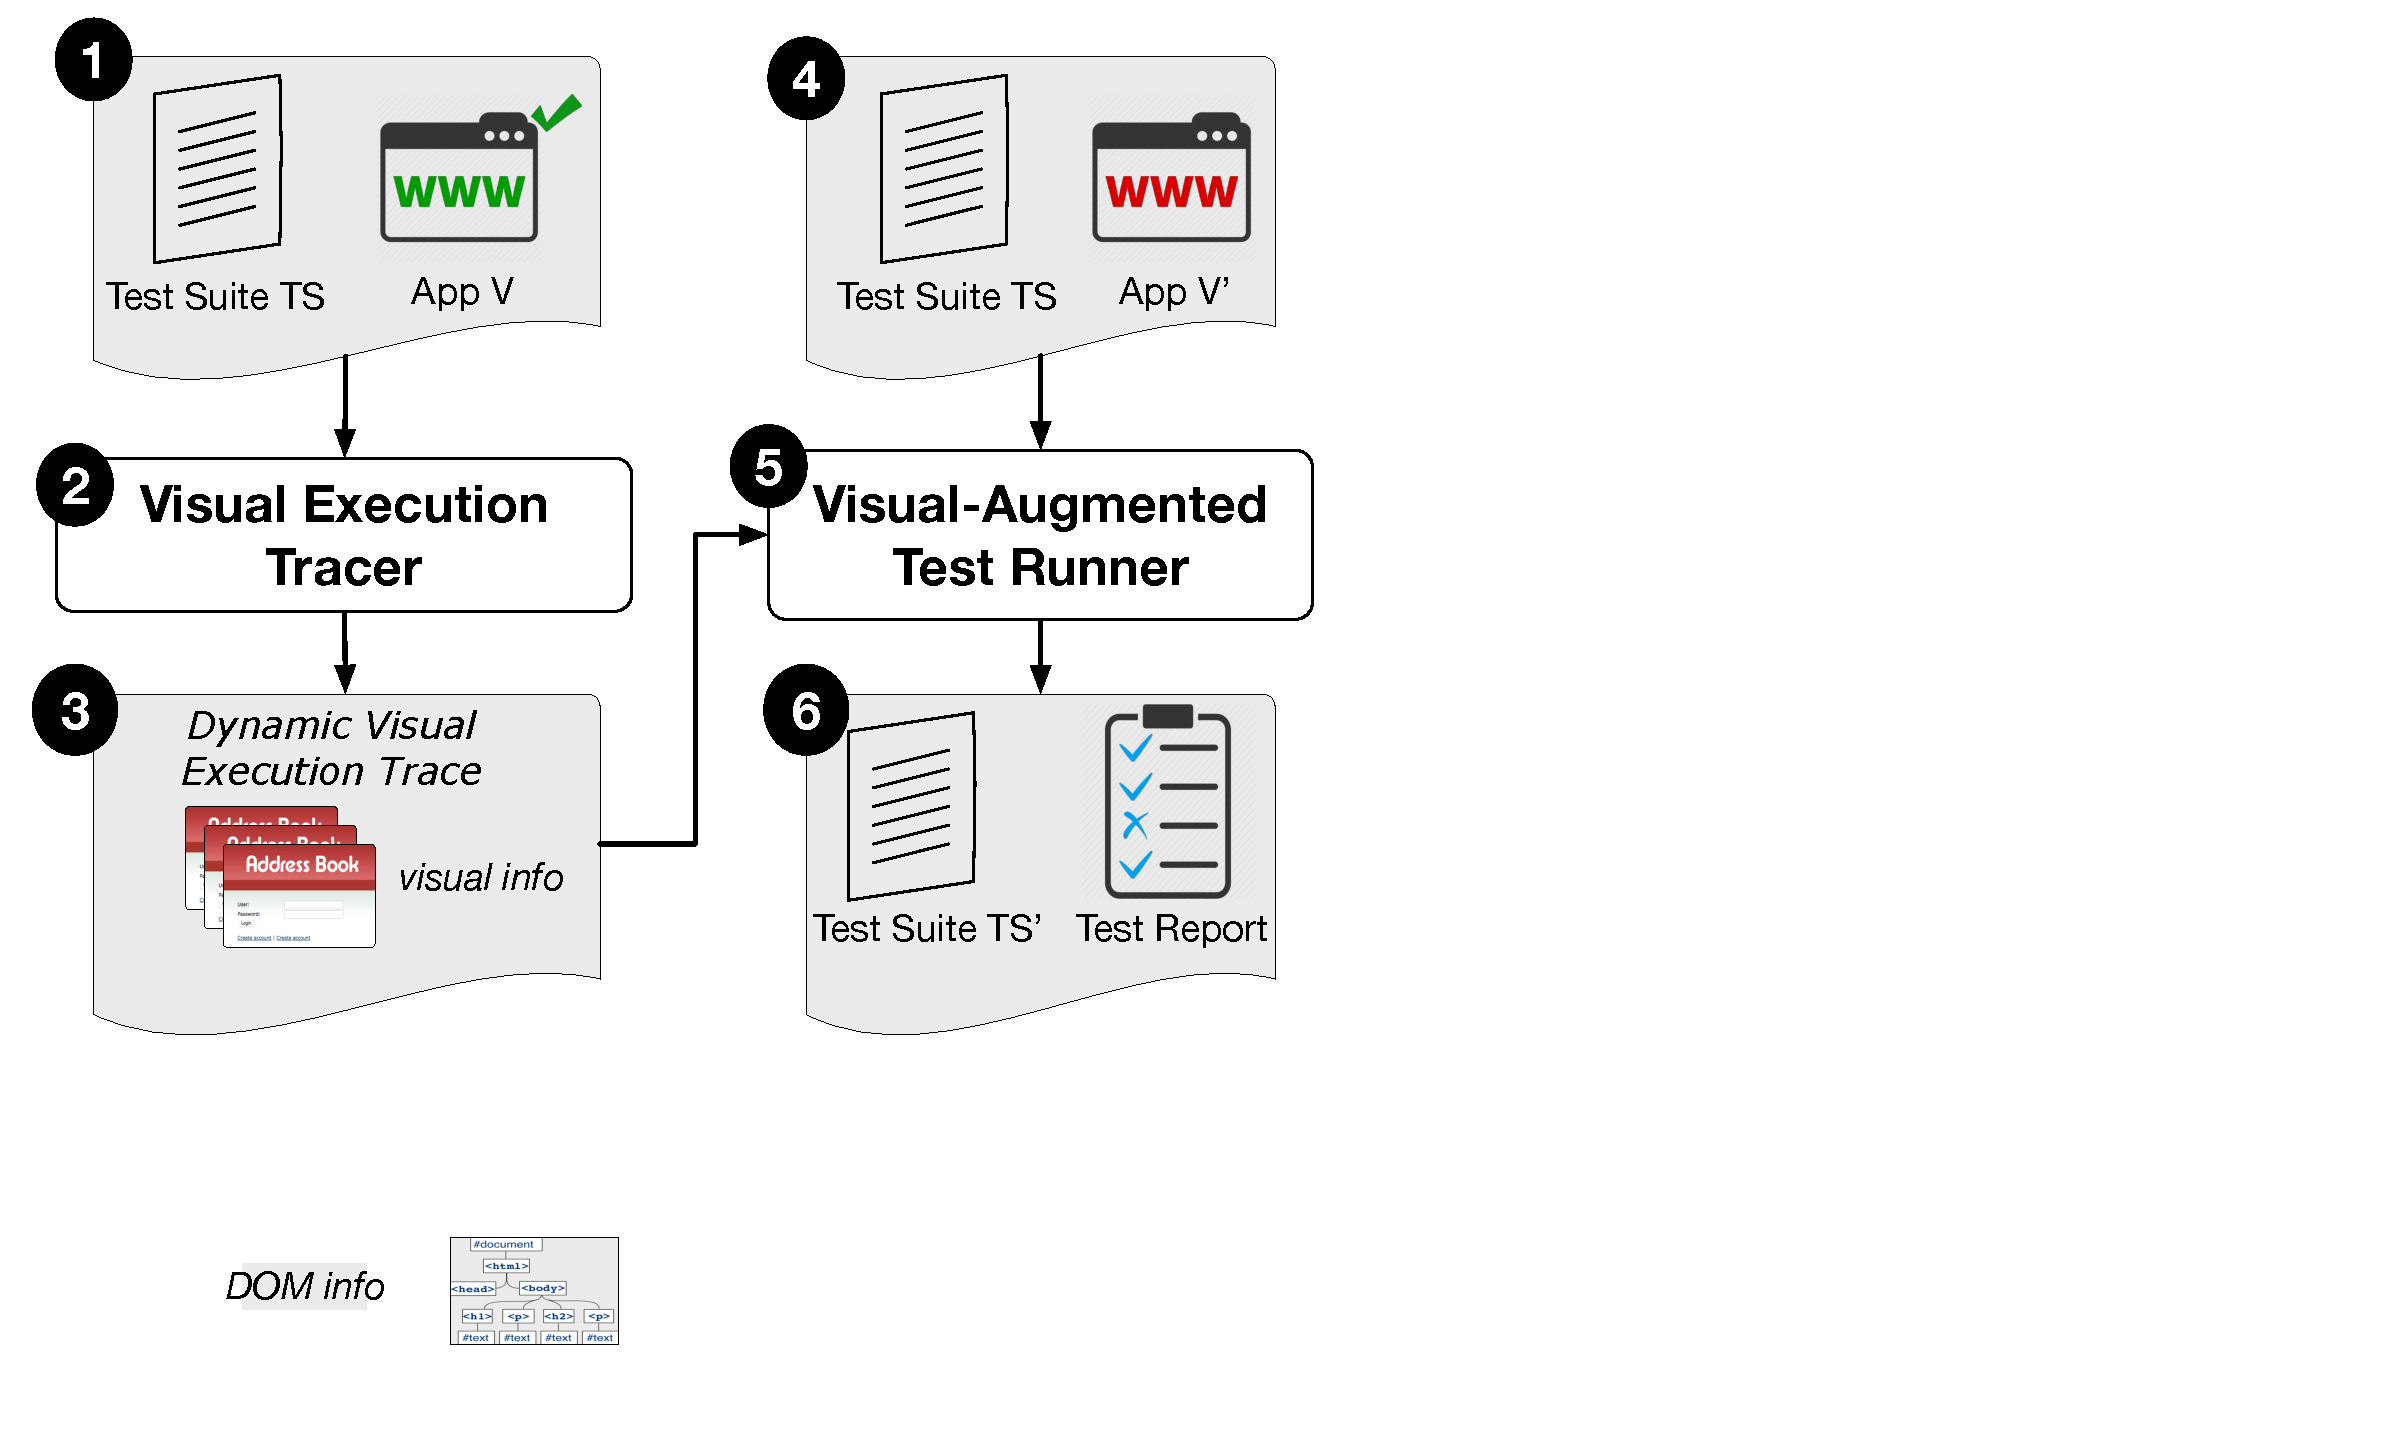
\includegraphics[trim={0.2cm 6.5cm 17cm 0.2cm},clip,scale=0.28]{images/approach-bigger}
%}
\caption{Overview of our approach}
\label{approach}
\end{figure}

%While most of the DOM information could be collected statically, the visual appearance of the rendered elements may change during the application execution and some elements may be not visible until specific events occur. For this reason, we need to capture the visual information at runtime, while the test suite is executing. 

%To this aim, the first module of \tool takes as input a web application along with its accompanying test suite, and runs each test case to collect both DOM and visual information associated to each test statement, hence creating a test model.  %\andrea{I haven't detailed this part by means of an algorithm as references are provided}

%We used and adapted the publicly available version of \textsc{PESTO}~\cite{2014-Stocco-SCAM}, a tool that uses aspect-oriented programming~\cite{aop} -- to intercept all Selenium WebDriver method calls (e.g., \texttt{click()}, \texttt{sendKeys()}, etc) using properly defined join-points. 

%We use aspect-oriented programming~\cite{aop} to intercept all Selenium WebDriver method calls (e.g., \texttt{click()}, \texttt{sendKeys()}, etc) using properly defined join-points. When a given join-point matches, advice methods store the test state \textit{before} and \textit{after} the statement's execution. 

More in detail, the test state encompasses the following DOM-related information: \textit{(d1)}~the DOM of the HTML page, \textit{(d2)}~the XPath of the web element the test statement interacted with and \textit{(d3)}~all its HTML attributes. The collected visual information concern: \textit{(v1)}~the screenshot, \textit{(v2)}~the coordinates and size of the web element's bounding box, and \textit{(v3)}~a visual locator for it. A visual locator is the portion of the rendered web page that uniquely identifies such web element on the screen~\cite{2015-Leotta-SAC}. 
%(Note that, as explained in~\cite{2014-Stocco-SCAM,2015-Leotta-SAC}, a visual locator is not always the precise crop of the web element's bounding box. There are cases in which a larger crop---taking into account the web element's visual context---is necessary in order to visually differentiate it from other visually similar web elements appearing on the page, as the case of a list of input text fields in a form).
%

\subsection{Visual-Augmented Execution}

\autoref{algo:alg1} illustrates the main procedure of our algorithm for the visual-augmented execution of test cases. The procedure takes as input a test case $T$, 
the dynamic visual execution trace $EX$ of $T$ on a version $V$ of the web application, and the URL $U$ of the web application $V'$. The outputs are a test $T'$, validated or corrected to work on $V'$, and the list of repairs. 

\noindent
\textbf{Initialization.} 
The initial part involves loading the previously saved trace execution information of the test $T$ on the reference version $V$, and loading the new version $V'$ by means of Selenium WebDriver (Lines~1--2). 

\noindent
\textbf{Visual-Augmented Execution.}
Such information is used to ``visually'' validate each statement $st_i$ of $T$, when executed on $V'$ (main loop Lines~4--36). The validation proceeds as follows. First, the DOM-based locator utilized by the test statement is extracted from $st_i$, along with the visual locator (e.g., an image) and the DOM information associated to the trace of $st_i$ in $V$  (Lines~5--7). Then, the \texttt{driver} instance is used to query the DOM of $V'$ to observe if the locator returns a web element (Line~8). 

\begin{algorithm}[b]
\scriptsize
\DontPrintSemicolon % Some LaTeX compilers require you to use \dontprintsemicolon instead
\KwIn{$T$: A test case developed for web application $V$, the URL $U$ of its subsequent version $V'$, $EX$: Execution Trace of $T$ when executed on $V$}
\KwOut{$T'$: A verified/repaired $T$ working on $V'$}
%\colorbox{lightgray}{/* Execution Trace collection */} \;
\textit{trace} $\gets$ loadExecutionTrace($EX$) \;
\textit{driver} $\gets$ loadApp($U$) \;
\textit{statements}, \textit{repairedStatements} $\gets$ getStatements(T) \;
 \ForEach{ test statement $st_i \in$ \textit{statements} }{%
  \textit{locator} $\gets$ getLocator($st_i$)\;
  \textit{\textit{visLocator}} $\gets$ getVisualLocator(\textit{trace}, $st_i$) \;
 \textit{\textit{DOMInfo}} $\gets$ getDOMInfo(\textit{trace}, $st_i$) \;
  \textit{webElement} $\gets$ \textit{driver}.findElement(\textit{locator})\;
  \HiLi{/* Manage non-selection of web element. */} \;
   \uIf{webElement == null} { 
     \textit{webElemVisual} $\gets$ \textsc{visualSearch}(\textit{driver}, $st_i$, \textit{visLocator}, \textit{DOMInfo})\;
     \uIf{\textit{webElemVisual} == null} {
       \textit{webElemVisual} $\gets$ \textsc{localCrawling}(\textit{driver}, $st_i$, \textit{visLocator}, \textit{DOMInfo})\;
       \uIf{\textit{webElemVisual} == null} {
       \textit{repairedStatements}.remove($st_i$)\;
       } \Else{
       \textit{newStmt} $\gets$ <\textsc{synthetizeLocator}(\textit{webElemVisual}), ``click'', ``''> \;
       \textit{repairedStatements}.addBefore($st_i$, \textit{newStmt}) \;
        }
     } \Else{
     updateLocator($st_i$, \textit{webElemVisual}) \;
      \textit{repairedStatements}.update($st_i$) \;
     }
   \HiLi{/* Manage mis-selection of web element. */} \;
   } \ElseIf{webElement $\neq$ null}{
      \textit{webElemVisual} $\gets$ \textsc{visualSearch}(\textit{driver}, $st_i$, \textit{visLocator}, \textit{DOMInfo})\;
     \textit{webElement} $\gets$ \textsc{verify}(\textit{webElement}, \textit{webElemVisual})\;
      \textit{repairedStatements}.update($st_i$, \textit{webElement}) \;
   }
   \HiLi{/* Suggest potential fix to assertions value. */} \;
    \If { webElement.getText() $\neq$ getTextualContent($st_i$) } {
         \textit{newStmt} $\gets$ <\textit{webElement}, ``getText'', webElement.getText()> \;
      	\textit{repairedStatements}.replace($st_i$,  \textit{newStmt}) \;
      }
         \textit{driver} $\gets$ \textsc{executeStatement}($st_i$, $V'$) \;
      	$T'$.add($st_i$) \;
 }
\Return{$T'$, \textit{repairedStatements}}\;
\caption{Overall Algorithm}
\label{algo:alg1}
\end{algorithm}

\noindent
\textbf{Detecting and Repairing Non-Selection problems.}
If no elements are returned, we treat it as a non-selection happening on the same state (\textit{Scenario 1}), and $st_i$ will break in $V'$, which we attempt to repair through a series of countermeasures. The first heuristic tries to search for the web element \textit{visually} on the same state. The \texttt{visualSearch} function (Line~11) uses advanced computer vision algorithms to retrieve the target web element visually by matching the visual locator captured in $V$ on the current screenshot of $V'$ (see details in \autoref{sec:vis}). The DOM information is also used to guide the search, and filter out potential outliers or visual false positives (such as visual duplicates). If a result is found, the locator of $st_i$ is updated, and the corrected statement saved in the list of repairs (Line~21--22). Then, $st_i$ saved as a statement of the new test case $T'$. Before to proceeding to the next statement, the approach outputs the outcome of the verification phase to the user, who can inspect, confirm and execute $st_i$, or enter a manual fix (for brevity, such details are encapsulated within the \texttt{executeStatement} function of Line~36).

If the visual search on the same state fails, then our approach assumes that the element no longer exists on the current state. We consider this a broken workflow and trigger a local exploration of the application state space (procedure \textsc{localCrawling} of Line~13) in order to find the element in the neighbouring states (\textit{Scenario 2}). In each new state discovered by the exploration, we attempt the \textsc{visualSearch} procedure to locate the element. If a match is found in at least one of those states, a new statement to reach that state (i.e, page) is created, with the corresponding DOM locator and a default \texttt{click} action, and added before $st_i$ in the the list of repairs (Lines~17--18).

On the contrary, if a match is \textit{not} found, i.e., no elements were found through local crawl, we attempt to repair the broken workflow by deleting $st_i$ (\textit{Scenario 3}) at Line~15.

\noindent
\textbf{Detecting and Repairing mis-selection problems.}
If a web element was returned by the original DOM-based locator, our approach asserts the correctness of the selection by using the previously collected visual and DOM information (Lines~25--29). 
The \texttt{verify} function checks the equivalence of the web elements found by the DOM-based and the visual locator. If they do differ, we consider it as a possible case of propagated breakage, the procedure reports the mismatch and stores the web element retrieved by the \texttt{visualSearch} function (Line~28).

\noindent
\textbf{Suggesting repairs to assertion values.}
Although the scope of the algorithm is to verify and correct locator issues, it is straightforward to check assertion values as well. Indeed, in case of the execution of $st_i$ raises an \texttt{AssertionError}, the new GUI value is saved and a statement with the new assertion value is created and saved in the repairs list (Lines~31--34). 
However, only a human tester can ascertain whether the assertion on new GUI value does reflect the intended application behaviour. Upon inspection, the tester can then either discard or accept the suggested repair.

\noindent
\textbf{Outputs.}
If \autoref{algo:alg1} terminates, our approach was able to either verify the statements of $T$ or provide candidate repairs for them. 
% in the new version $V'$. 
If $T = T'$ no regressions have occurred, otherwise $T'$ and the list of repairs are returned.
If \autoref{algo:alg1} stops prematurely, then one of the statements executed by the function \textsc{executeStatement} triggered an action that could not be performed or an incorrect locator was retrieved. The tester must then intervene to manually correct such unfortunate cases.

In the following sections we describe the core components of our algorithm, that is the \textsc{visualSearch} and \textsc{localCrawling} procedures that underlie at the functioning of our approach.

\subsection{Visual Search of Web Elements}\label{sec:vis}

One of our motivations of conducting this research is to use computer vision (CV) techniques to assist software-engineering tasks. 
Thereby, we provide a short background of the CV solutions that are useful in our setting.

\noindent
\textbf{Challenges of Template Matching.}
Identifying web elements \textit{visually} across different versions (i.e., pages) of a web application falls within a common branch of image analysis known as \textit{template matching}. 
%
Template matching aims to detect the occurrence of a specific object image (template) in another image~\cite{Brunelli:2009:TMT:1643435}. The template is slid over the image, and a a similarity measure is computed at each pixel location.
%This is done by defining a small image of the object, a template, and searching for a similar occurrence in a given image, by sliding the template over the image, and computing a similarity measure at each pixel location.
%
In our context, our matching technique must handle \textit{translation} (i.e., the captured template can be shifted with respect to the reference image) and \textit{scaling} (i.e., the aspect ratio of the template is not preserved in the reference image, or a different font is used) problems. Indeed, web applications are often modified to accommodate cosmetic or stylistic changes to align the GUI with the latest trends. These changes may render our technique fragile, because the visual locators captured on the `old' GUI might be ineffective on the GUI of the new application. Additionally, standard template matching algorithms are not effective in detecting the presence/absence of a template, which is instead of paramount importance for the accuracy our algorithm.
Even if stricter threshold values might be used, in practice this is not robust or generalizable, thus we explored feature detection and key-point matching algorithms.

\begin{figure}[t]
\centering
%\fbox{
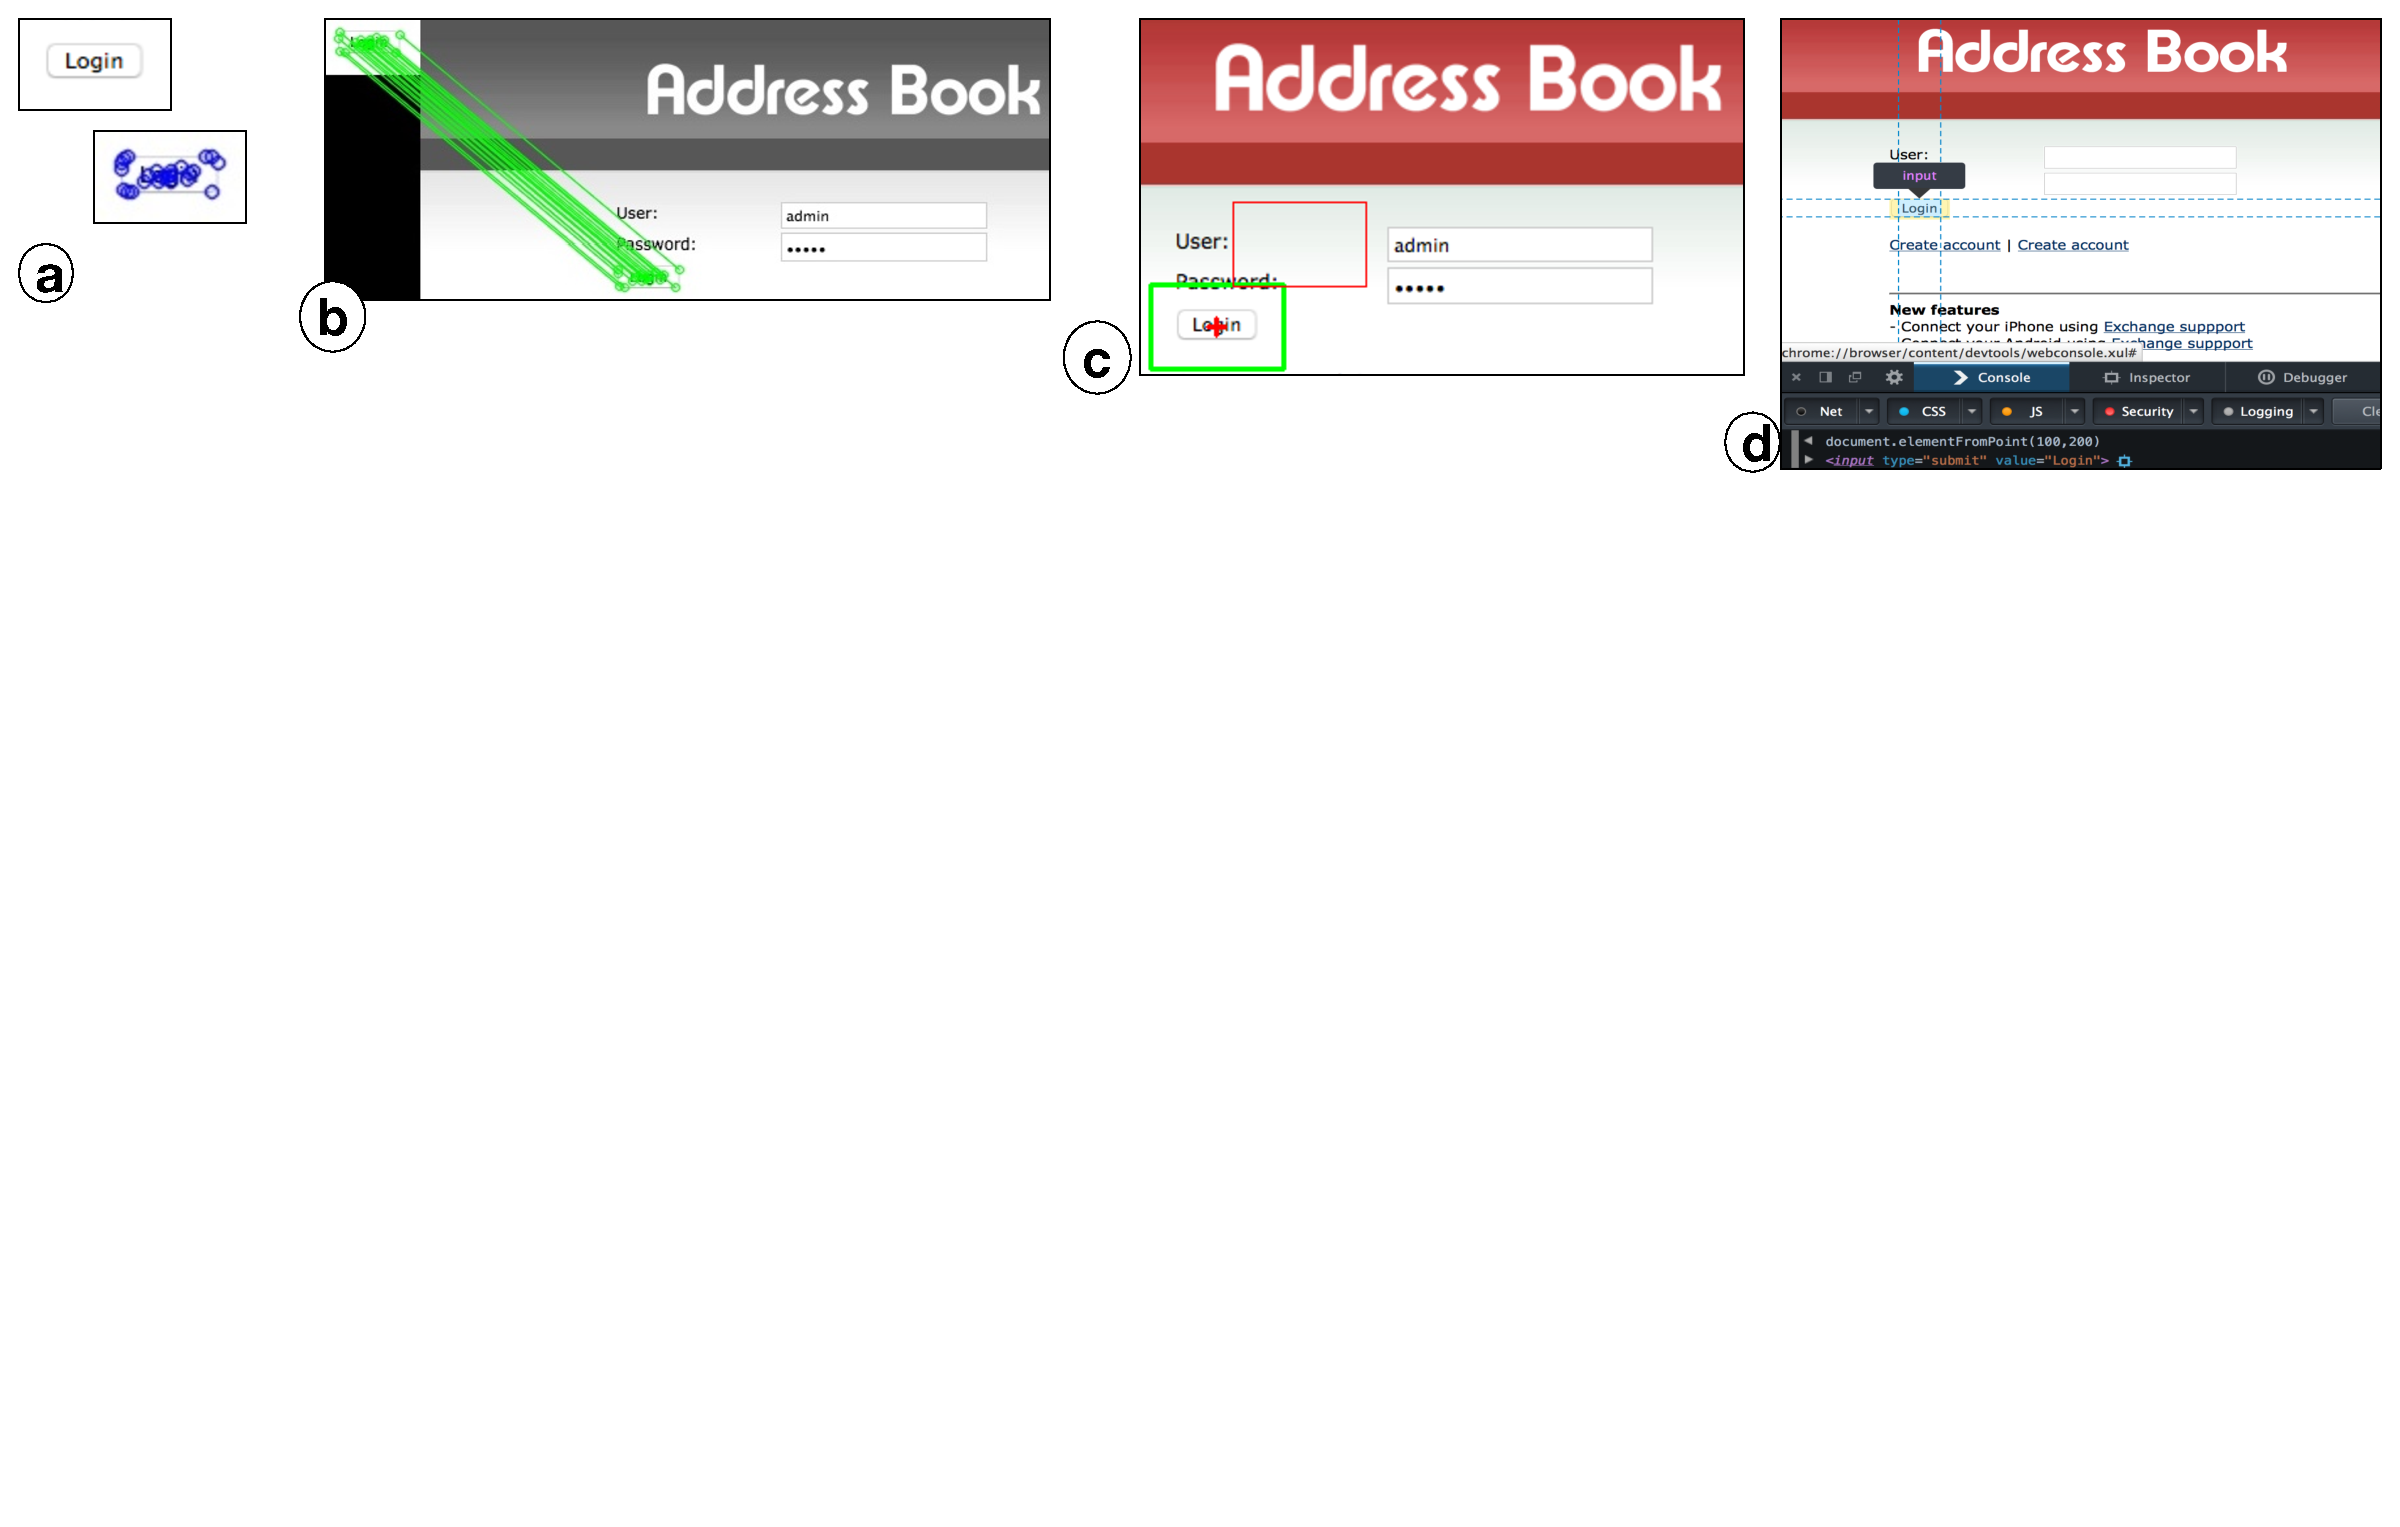
\includegraphics[trim={0cm 0cm 0cm 0cm},clip,scale=0.18]{images/cv}
%}
\caption{Computer vision pipeline for robust web element detection.}
\label{fig:cv}
\end{figure}

\noindent
\textbf{Feature Detection.}
The philosophy of this method is to find certain ``important'' points (\textit{key-points}) in the  template image and store information about the neighbourhood of those key-points (\textit{key-point descriptors}) as a description of the template. Then, after finding the descriptors of key-points in the reference image, the algorithm tries to `match' the two descriptor sets (one from the template and one from the reference image) using some notion of similarity, and see how many descriptors match.

Thus, the \textsc{visualSearch} adopts a pipeline of CV algorithms, each one devoted to a specific task. The pipeline is graphically illustrated in \autoref{fig:cv}. 

\noindent
\textbf{Feature Detection for Template Absence/Presence.}
In order to robustly detect the absence/presence of the template image in a web page, we adopted two famous feature detection algorithms from the CV literature, SIFT~\cite{Lowe1999,Lowe2004} and FAST~\cite{rosten2005tracking,rosten2008faster}, to detect the key-points from the template image~\textcircled{\raisebox{-0.6pt}{a}}. 
Through experimentation, we found that these two approaches complement each other. As such, SIFT performs well mostly for text-based templates whereas FAST can handle the cases where the template represents an ``empty'' text field, as it is specifically designed for corner detection. In our pictorial example~\textcircled{\raisebox{-0.6pt}{a}}, most of the key-points detected by SIFT are in fact nearby the ``Login'' label (orange circles), whereas FAST detected key-points also in proximity of the corners (blue circles). In ~\textcircled{\raisebox{-0.6pt}{b}} we can see how the algorithms matched the key-points onto the new web page.
 
%Then, descriptors are calculated for each key-point, and the algorithms try to match them onto the new screenshot by identifying their nearest neighbours~\textcircled{\raisebox{-0.6pt}{b}}. 
%We set the algorithm's threshold to $\gamma=0.8$ (as suggested by Lowe's paper~\cite{Lowe1999}), to decide upon rejection of matches.
%If at least 80\% of key-points are matched across the two images, we can have a certain degree of confidence that the template is present in the image. 

\noindent
\textbf{Template Matching with Visual Filtering.}
In the next step, if the feature detection returned a positive result about the presence of the template image, a template matching technique is executed~\textcircled{\raisebox{-0.6pt}{c}} (specifically, we used the Fast Normalized Cross Correlation algorithm~\cite{briechle2001template}). 
%The performance of template matching oscillates depending on various factors, such as the size or the aspect ratio of the template. 
If multiple visual matches are found, those that do not fall in the region where most of the key-points have been found, are discarded (\textit{visual-based filtering}). 
%If multiple matches are still present, we retrieve the DOM elements corresponding to each match, and we calculate the closest web element that matches the DOM information (\textit{DOM-based filtering}).
Thus, only the closest match is returned (see the green thick rectangle over the ``Login'' button). In brief, the three algorithms operate to find a consensus on the location area of the best match.

\noindent
\textbf{From GUI to DOM.}
To retrieve the DOM-element corresponding to a specific point of coordinates $(x,y)$, \textsc{visualSearch} queries the browser through JavaScript 
%command -- \texttt{elementFromPoint(x,y)} -- that returns the 
to get the DOM element whose bounding box contains \texttt{x} and \texttt{y}~\textcircled{\raisebox{-0.6pt}{d}}.

%To precisely identify the web element of interest, we need to provide the function with the coordinates of the the \textit{centre} of the bounding box. Otherwise, a DOM ancestor of the searched web element (e.g., the \texttt{form} container), will be erroneously retrieved.

\subsection{Local Crawling for Workflow Repair}

Manually repairing every broken workflow is tedious and frustrating, since even a medium-size web application may contain tens of GUI screens and hundreds of GUI actions. It is hence likely infeasible for a tester to quickly explore this space to choose replacement actions from.

Fortunately, a web crawler can do this automatically. To this end, the \texttt{localCrawling} function features \textsc{Crawljax}, a state of the art tool for the automatic crawling of dynamic web applications~\cite{mesbah:tweb12,mesbah:tse12}. We developed a \textsc{Crawljax} plugin that incorporates the \texttt{visualSearch} function (Line~11), so that the crawler can effectively explore the state space of $V'$ looking for a visual match in all the neighbouring states of the current test state (Line~13). As a conservative choice, since the number of DOM states and events can be numerous, we set the crawling depth to one (1). On the one hand, this limits the search capability, potentially missing states in which the elements could be found. On the other hand, this choice keeps the running time acceptable.

\subsection{Implementation}\label{sec:implementation}

We implemented our approach in a tool called \tool, which is publicly available (URL omitted). 
The tool is written in Java, and supports Selenium test suites written in Java. However, our overall approach is more general and applicable to test suites developed using other programming languages or testing frameworks. 
\tool gets as input the path to the test suites, collects the visual execution traces by means of \textsc{PESTO}~\cite{2014-Stocco-SCAM}, runs the visual-augmented detection and repair algorithm using the computer vision libraries available in OpenCV~\cite{opencv}, and \textsc{Crawljax}~\cite{mesbah:tweb12,mesbah:tse12} for the local crawling exploration. 
\tool makes use of the traces to generate potential repairs and generates a list of repaired test cases.







